\documentclass{report}

%------------------------------------------------------------
% All packages are here defined
%------------------------------------------------------------

\usepackage[a4paper]{geometry}
\usepackage{vmargin}
\usepackage[english]{babel}
\usepackage[english]{varioref}
\usepackage[utf8]{inputenc}
\usepackage{graphicx}
\usepackage{array}
\usepackage{float}
\usepackage{tabularx}
\usepackage{hhline}
\usepackage{amsmath}
\usepackage{hyperref}
\usepackage{url}
\usepackage{fancyhdr}
\usepackage{setspace}
\usepackage{listings}
\usepackage{color}
\usepackage{abstract}
\usepackage{titlesec}
\usepackage{multirow}
\usepackage{datetime}
\usepackage{varwidth}

%----------------------------------------------------
%	MARGINS
%----------------------------------------------------
\setmarginsrb  { 1.5in}  % left margin
                        { 0.6in}  % top margin
                        { 1.0in}  % right margin
                        { 0.8in}  % bottom margin
                        {  20pt}  % head height
                        {0.25in}  % head sep
                        {   9pt}  % foot height
                        { 0.3in}  % foot sep
%----------------------------------------------------------------------------------------

%-------------------------------------------------
% Colors defination
%--------------------------------------------------
\definecolor{dkgreen}{rgb}{0,0.6,0}
\definecolor{gray}{rgb}{0.5,0.5,0.5}
\definecolor{mauve}{rgb}{0.58,0,0.82}
\definecolor{navyblue}{rgb}{0.0, 0.0, 0.5}



%-------------------------------------------------
% language settings for code insertion
%---------------------------------------------------
\lstset{frame=tb,
  language=Java,
  aboveskip=3mm,
  belowskip=3mm,
  showstringspaces=false,
  columns=flexible,
  basicstyle={\small\ttfamily},
  numbers=none,
  numberstyle=\tiny\color{gray},
  keywordstyle=\color{blue},
  commentstyle=\color{dkgreen},
  stringstyle=\color{mauve},
  breaklines=true,
  breakatwhitespace=true
  tabsize=3
}

%----------------------------------------------------------
% Horizontal line formation
%--------------------------------------------------------
\newcommand{\Hline}{\par
  \begin{center}
   \line(1,0){400}
   \end{center}
}


%------------------------------------------------------
% heading formation for chapters and other headings
%------------------------------------------------------
\titleformat
{\chapter} % command
[display] % shape
{\bfseries\LARGE} % format
{\Huge{Chapter.\ \thechapter}} % label
{0.5ex} % sep
{
\rule{\textwidth}{1pt}%
\vspace{1ex}
\centering
} % before-code
[
\vspace{-0.5ex}%
\rule{\textwidth}{0.3pt}
] % after-code

%-------------------------------------------------------
%heading formation for Acknowledgement
%-------------------------------------------------------


%---------------------------------------------------------
% Others
%----------------------------------------------------------

\newdateformat{mydate}{\monthname[\THEMONTH] \THEYEAR}	
%\geometry{a4paper}
\renewcommand{\abstractnamefont}{\normalfont\LARGE\bfseries}


%------------------------------------------------------
% Beginning main document
%---------------------------------------------------

\begin{document}
\pagenumbering{gobble} 


%----------------------------------------------------------------------------------------
%	Title page
%----------------------------------------------------------------------------------------
\begin{titlepage}
\begin{center}


{\huge \bfseries Graph Theoretical Algorithms For }\\[0.3cm]
{\huge \bfseries Structural Comparison Of Java Source}\\[0.3cm] % Thesis title
{\huge \bfseries  And Byte Code }\\[0.3cm]
\Hline

\begin{center}
\large{Submitted By}\\[0.2cm]
\textbf{\Large{Artem Garishin}}\\[2cm]
\end{center}


\includegraphics[width=0.50\textwidth]{Figures/FH_logo}\\[0.5cm]
\textbf{\large FB2: Faculty of Computer Science and Engineering}\\[1cm]


\large \textit{This thesis presented for the degree of\\ Master of Science} \\
\textit{in the}\\[0.2cm]
\textbf{\textcolor{navyblue}{High Integrity Systems}}\\[2.5cm] % Research group name and department name

\begin{center}


\begin{varwidth}{0.8\textwidth}
\raggedright
\textbf{Research Supervisor}: {Prof. Dr. Alekseev Sergej}\\[0.2cm] % Supervisor name - remove the \href bracket to remove the link  
\textbf{Co-Supervisor}: {Prof. Dr. Matthias Wagner}\\ % Supervisor name - remove the \href bracket to remove the link  
[3cm]
\end{varwidth}\\[3cm]
\end{center}



{\large \mydate\today}\\[1cm] % Date
%\includegraphics{Logo} % University/department logo - uncomment to place it

\vfill

\end{center}

\end{titlepage}


%----------------------------------------------------------
%Declaration
%---------------------------------------------------------
\doublespacing
\null\vfil
%\vskip 60\p@
\begin{center}{\huge\bf Legal Declaration\par}\end{center}
%\vskip 60\p@
\null
I declare that this thesis document is completely my own work and all used references have been clearly cited. I have not submitted this assignment in the context of an examination to any other examination board or person.\\[2.5cm]

\begin{flushleft}
Signature:\\
\rule[1em]{25em}{0.5pt} % This prints a line for the signature
 
Location, Date:\\
\rule[1em]{25em}{0.5pt} % This prints a line to write the date
\end{flushleft}


%-----------------------------------------------------------------
% Abstract 
%----------------------------------------------------------
\newpage
\pagestyle{fancy}
\fancyhead{}
\renewcommand{\headrulewidth}{0pt}
\renewcommand{\footrulewidth}{0.4pt}
\pagenumbering{Roman}
%\doublespacing
\begin{abstract}
\large
Java code is compare we need for ...

\par Why we need it


\par This paper also explains the existing ...
\end{abstract}

%--------------------------------------------------------
%Acknowledgement
%-------------------------------------------------------
\newpage
%\null\vfil
%\vskip 60\p@
\begin{center}{\huge\bf Acknowledgments\par}\end{center}
%\vskip 60\p@
\null
I would like to take this time to thank Frankfurt University of Applied Sciences for all of the resources which they provided me in order to pursuing my master study in computer science and make this thesis possible.\vspace{5 mm}

\noindent I would like to express my sincere gratitude to Prof. Dr. Sergej Alekseev and Prof. Dr. Matthias Wagner for their patient guidance, encouragement and advice which they provided me throughout this thesis work.

%----------------------------------------------------------------------
% Some configurations
%-------------------------------------------------------

\newpage
\tableofcontents
\listoffigures
\listoftables

%--------------------------------------------------------
%Abbreviations
%-------------------------------------------------------
\newpage
\setstretch{1.5}
%\null\vfil
%\vskip 60\p@
\Hline
\begin{center}{\huge\bf Abbreviations\par}\end{center}
\Hline
%\vskip 60\p@
\vspace{10mm}
\null

\noindent
\textbf{IEDAE} \hspace{20 mm} \textbf{I}nteractive \textbf{E}xploratory \textbf{D}ata \textbf{A}nalysis \textbf{E}nvironment\\
\textbf{SQL} \hspace{25 mm} \textbf{S}tructural \textbf{Q}uery \textbf{L}anguage \\
\textbf{API} \hspace{25 mm} \textbf{A}pplication \textbf{P}rogramming \textbf{I}nterface \\
\textbf{CI} \hspace{28 mm} \textbf{C}ontinuous \textbf{I}ntegration \\
\textbf{JDBC} \hspace{22 mm} \textbf{J}ava \textbf{D}ata \textbf{B}ase \textbf{C}onnectivity \\
\textbf{MVC} \hspace{23 mm} \textbf{M}odel \textbf{V}iew \textbf{C}ontroller \\
\textbf{HTML} \hspace{20.5 mm} \textbf{H}yper \textbf{T}ext \textbf{M}arkup \textbf{L}anguage \\
\textbf{XML} \hspace{23.5 mm} \textbf{E}xtensible \textbf{M}arkup \textbf{L}anguage \\
\textbf{JAXB} \hspace{22 mm} \textbf{J}ava \textbf{A}rchitecture for \textbf{X}ML \textbf{B}inding \\
\textbf{UML} \hspace{23.5 mm} \textbf{U}nified \textbf{M}odeling \textbf{L}anguage \\
\textbf{URL} \hspace{24.5 mm} \textbf{U}niform \textbf{R}esource \textbf{L}ocator \\
\textbf{HTTP} \hspace{21.5 mm} \textbf{H}yper \textbf{T}ext \textbf{T}ransfer \textbf{P}rotocol \\
\textbf{SCM} \hspace{24.5 mm} \textbf{S}ource \textbf{C}ode \textbf{M}anagement \\
\textbf{CVS} \hspace{25 mm} \textbf{C}oncurrent \textbf{V}ersion \textbf{S}ystem \\



%----------------------------------------------------------
% 1st Chapter
%------------------------------------------------------

\newpage
\pagenumbering{arabic}
\doublespacing
\large

\chapter{Introduction}
 This is 1st chapter
 
\section{Section}
This is section heading

\subsection{Sub Section}
This is sub section


%----------------------------------------------------------------------
% 2nd Chapter
%-----------------------------------------------------
\newpage	
\chapter{Current Scenario}
This is second chapter

\section{Background}
Here is way that how to reference from bibliography.
Giving references like this \cite{ch21}.


\section{Flow of the Project}

Here is way to put figure and its reference in document. 


Figure \ref{flow} shows the overall flow of the project.

\begin{figure}[h!]
\centering
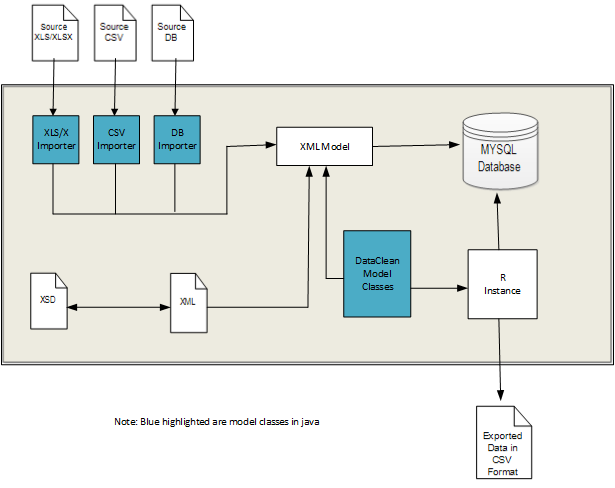
\includegraphics[width=1.0\textwidth]{Figures/flow}
\caption{Flow of the Project}
\label{flow}
\end{figure}

\newpage
\newpage
\par Here is a way to design table and put reference of a table
Table \ref{importclasses} gives visual overview of sequence in import process.

\begin{table}[h]
\centering
\begin{tabular}{|l|l|}
\hline
\multicolumn{1}{|c|}{\textbf{Items}}                     & \multicolumn{1}{|c|}{\textbf{Action}}                                                                                                                                                                                                                                            \\ \hline
DataImportCSVXLS (doimport)        & fileImport()                                                                                                                                                                                                                                                               \\ \hline
DataImportCSVXLS (fileimport)      &                                                                                                                                                                                                
newLoad().doLoad()
\\ \hline
Load (Constructor)                 & ImportFactory.getFrameWork(tcm)                                                                                                                                                               \\ \hline
ImportFactory (getFrameWork)       & \begin{tabular}[c]{@{}l@{}}csv =\textgreater return new ImportCSV(tcm)\\ xls/xlsx =\textgreater return new ImportExcel(tcm)\\ accdb/mdb =\textgreater return new ImporFromDB(tcm)\end{tabular}
\\ \hline
Load (Constructor)                 & \begin{tabular}[c]{@{}l@{}}Load has subclass instance of ImportFrameWork\\ instance.getInsert()\end{tabular}                                                                                    \\ \hline
ImportFrameWork (getInsert)        & \begin{tabular}[c]{@{}l@{}}getInsert is responsible for the insert and returns \\the list of insert commands back\\ generateLoadStatement()\end{tabular}                                          \\ \hline
ImportXXX,(generateLoad,Statement) & \begin{tabular}[c]{@{}l@{}} An instance of sub class, generates List and returns \\ it back
\end{tabular}                                                                                                                                      \\ \hline
ImportFramework,(getInsert)        &                                                                                                                                                                                                    
A list will be returned 
\\ \hline
Load (Constructor)                 & \begin{tabular}[l]{@{}l@{}}List will be imported into database, iterate over \\ the list \\ super.execute(command)\end{tabular}                                                                    \\ \hline
\end{tabular}
\caption{Classes and functions in import process}
\label{importclasses}
\end{table}

\newpage
\par Here is way to itemize the points with numbers

\begin{enumerate}
\item point 1
\item point 2
\end{enumerate}

\newpage
\par Here is way to itemize the points with bullets

\begin{itemize}
\item point 1
\item point 2
\end{itemize}

\newpage

\par Here is way to put code inside listing

\begin{lstlisting}
public class Main(){
	public static void main(String[] args){
	
	}
}
\end{lstlisting}



\newpage

%\bibliographystyle{plain}
\begin{thebibliography}{100} % 100 is a random guess of the total number of references 
\addcontentsline{toc}{chapter}{Bibliography}
\bibitem{ch11} George H.L. Fletcher and Catharine M. Wyss, ``Data Mapping as Search", Computer Science Department, School of Informatics, Indiana University, Bloomington, USA. 
 
\bibitem{ch12} Bogdan Alexe, Laura Chiticariu, Renee J. Miller, Wang-Chiew Tan, ``Muse: Mapping Understanding and deSign by Example", University of California, Santa Cruz, University of Toronto. 
 
\bibitem{ch21} Dorian Pyle, ``Data Preparation for Data Mining".
 
\bibitem{ch22} Erich Teichmann, Eren Demir, Thierry Chaussalet, ``Data preparation for clinical data mining to identify patients at risk of readmission", Department of Information Systems and Computing, School of Informatics, University of Westminster, London, W1W 6UW, UK.
\end{thebibliography} 

\end{document}
